\documentclass[final]{report}
\usepackage{graphicx}


\begin{document}

\title{Test Procedure for \\
  Nanometric Discriminator Cards \\
  for Wire Chambers}

\date{July 17, 2015}

\author{James Clarke,\\
Mitchell Kerver,\\
Christian Davison }

\maketitle

\begin{figure}[1]
  \centering
  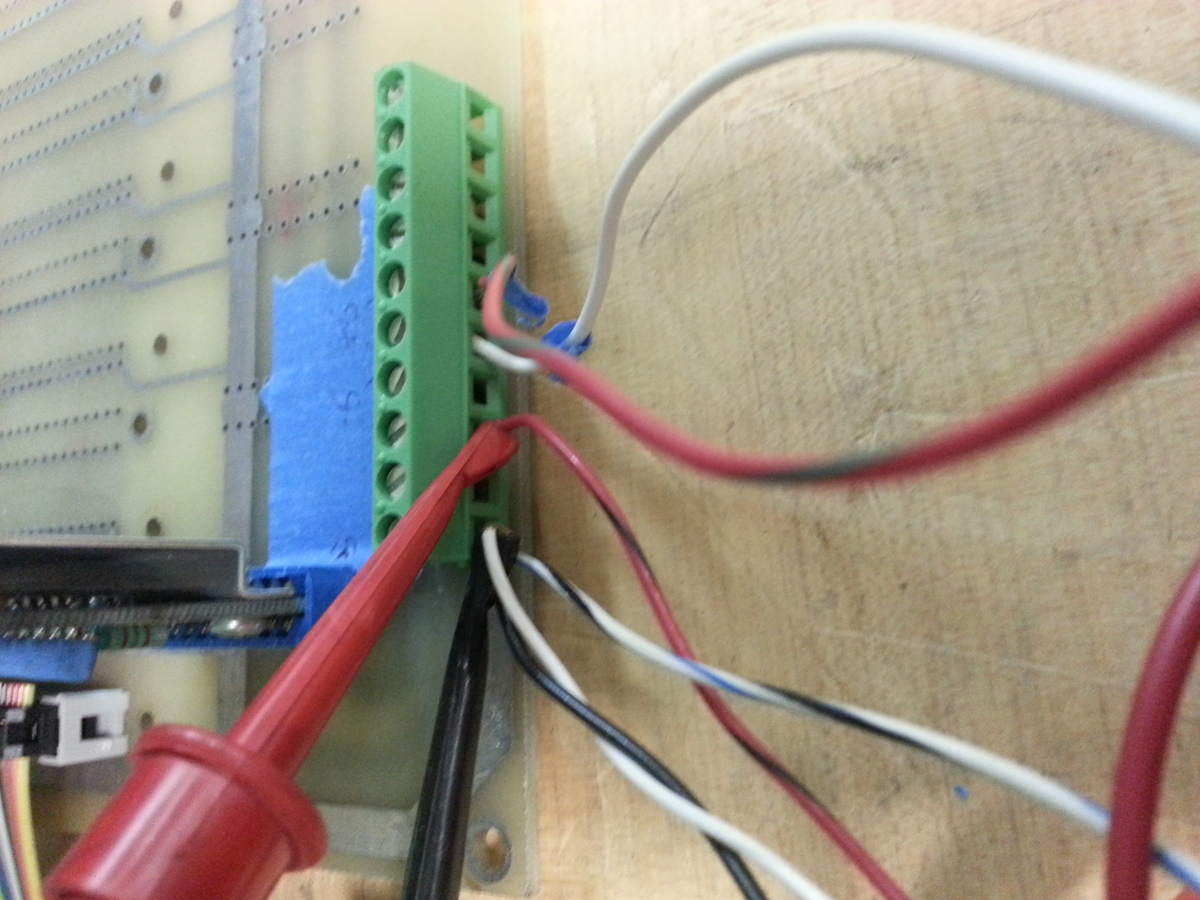
\includegraphics[height=3in, angle = -90]{Figure1.jpg}
  \caption{The various voltage sources going into the circuit board. Note all three grounds going into a common slot and the voltmeter attached to the threshold source wires}
  \label{fig:bus}
\end{figure}
\begin{figure}[2]
  \centering
  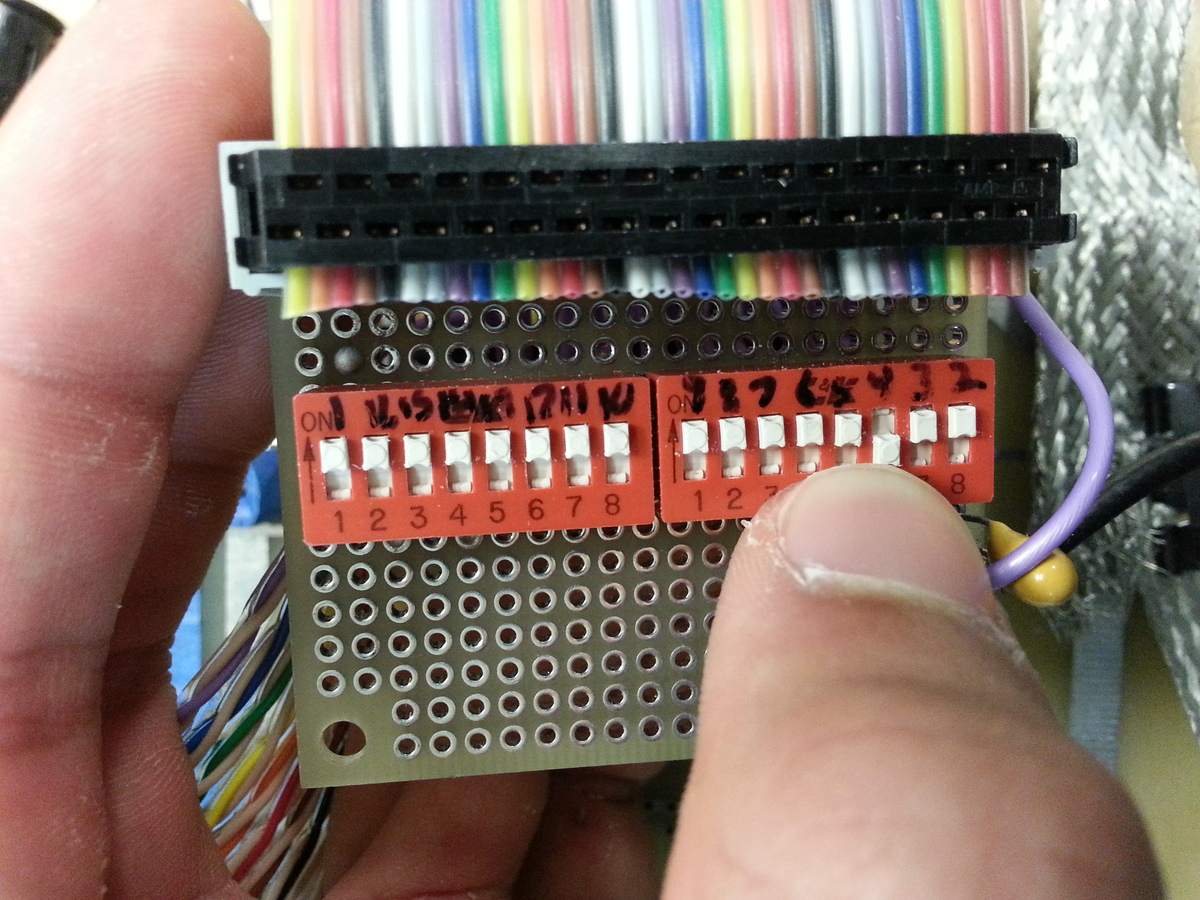
\includegraphics[height=3in]{Figure2.jpg}
  \caption{The sixteen switches with channel four in the off position. On this particular board, the channels are a little messed up with one coming first then the rest of the numbers in reverse order from 16 to 2.}
  \label{fig:switches}
\end{figure}
\begin{figure}[3]
  \centering
  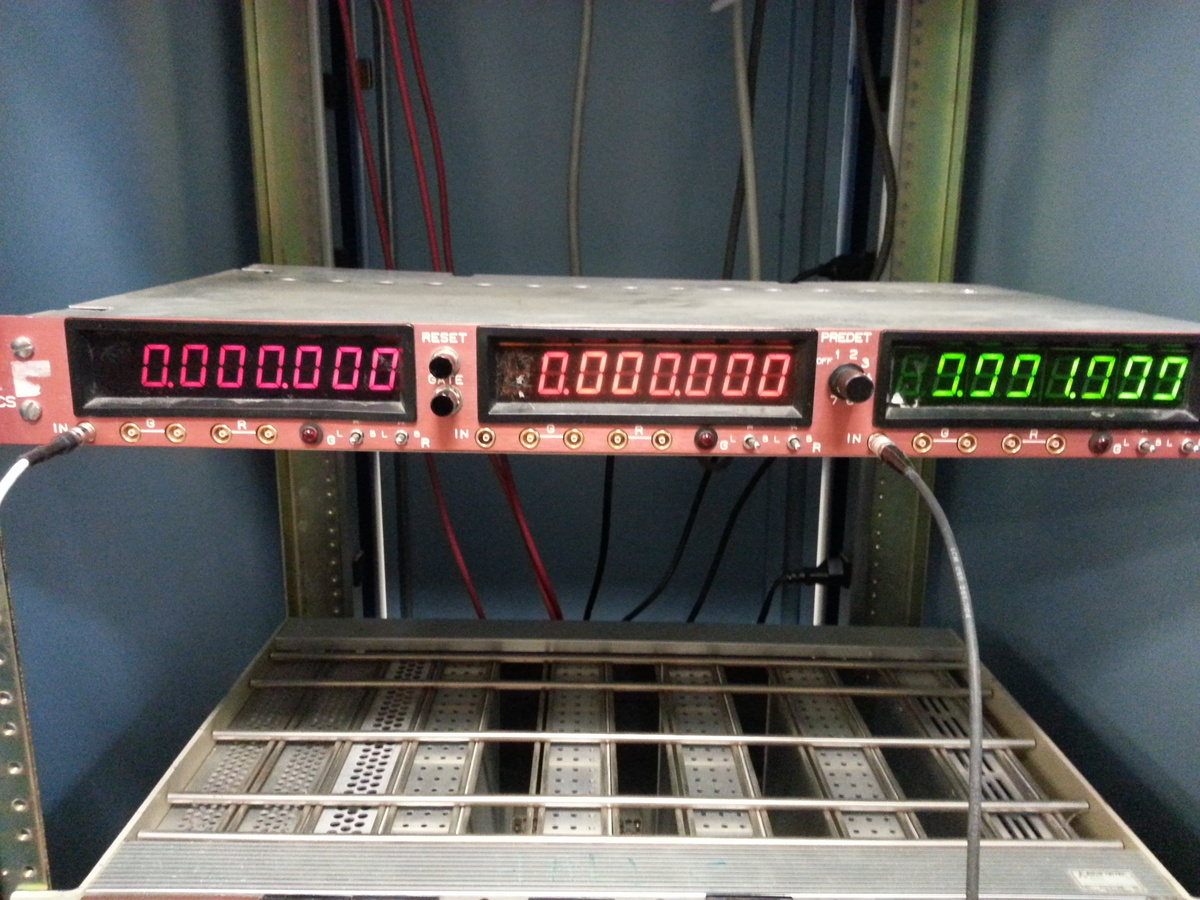
\includegraphics[height=3in]{Figure3.jpg}
  \caption{The scaler model we used. The card signal from the NIM module is the left wire, while the test pulse is in the right input}
  \label{fig:scaler}
\end{figure}
\begin{figure}[4]
  \centering
  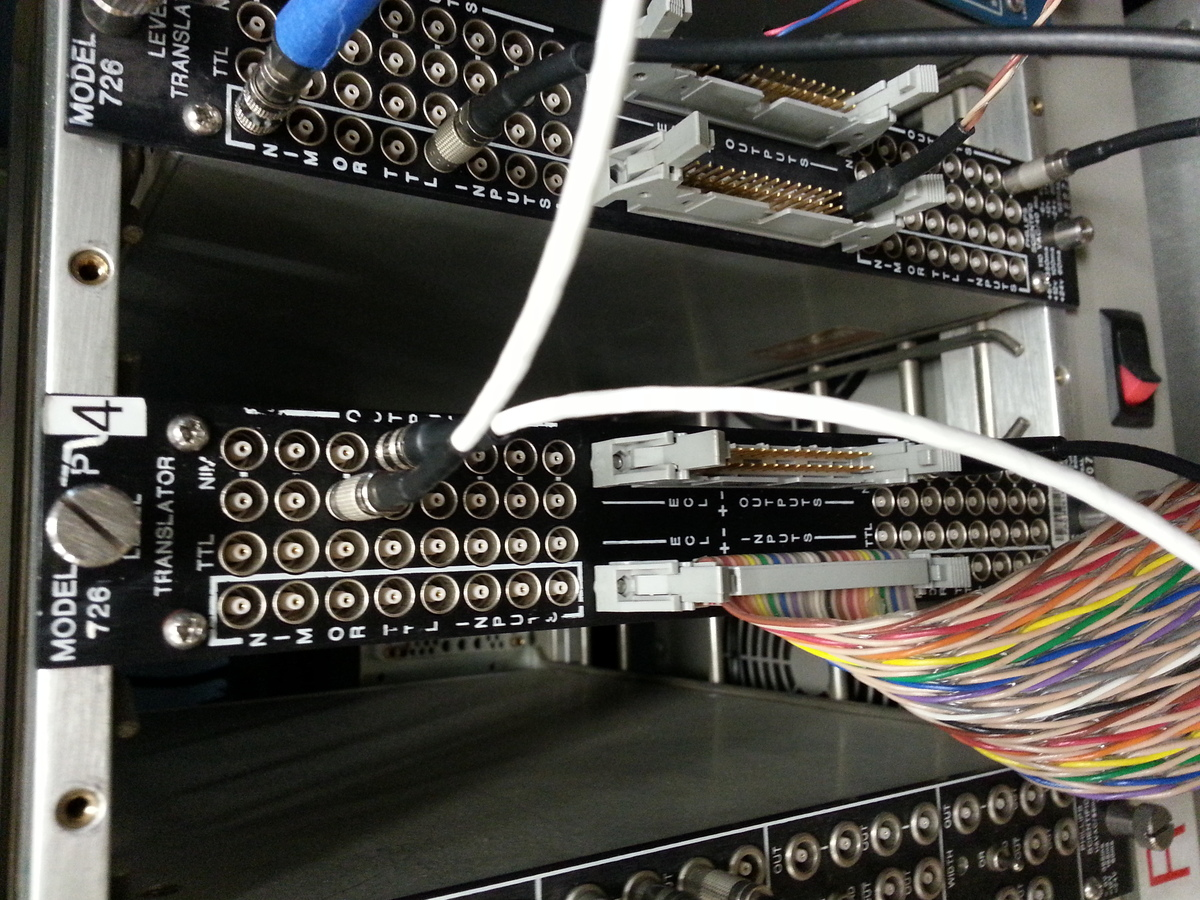
\includegraphics[height=3in, angle = -90]{Figure4.jpg}
  \caption{The NIM module. The ribbon cable is the input. The cable in channel 3 goes to our oscilloscope while the cable in channel 4 goes to our scaler}
  \label{fig:nimboard}
\end{figure}
\begin{figure}[5]
  \centering
  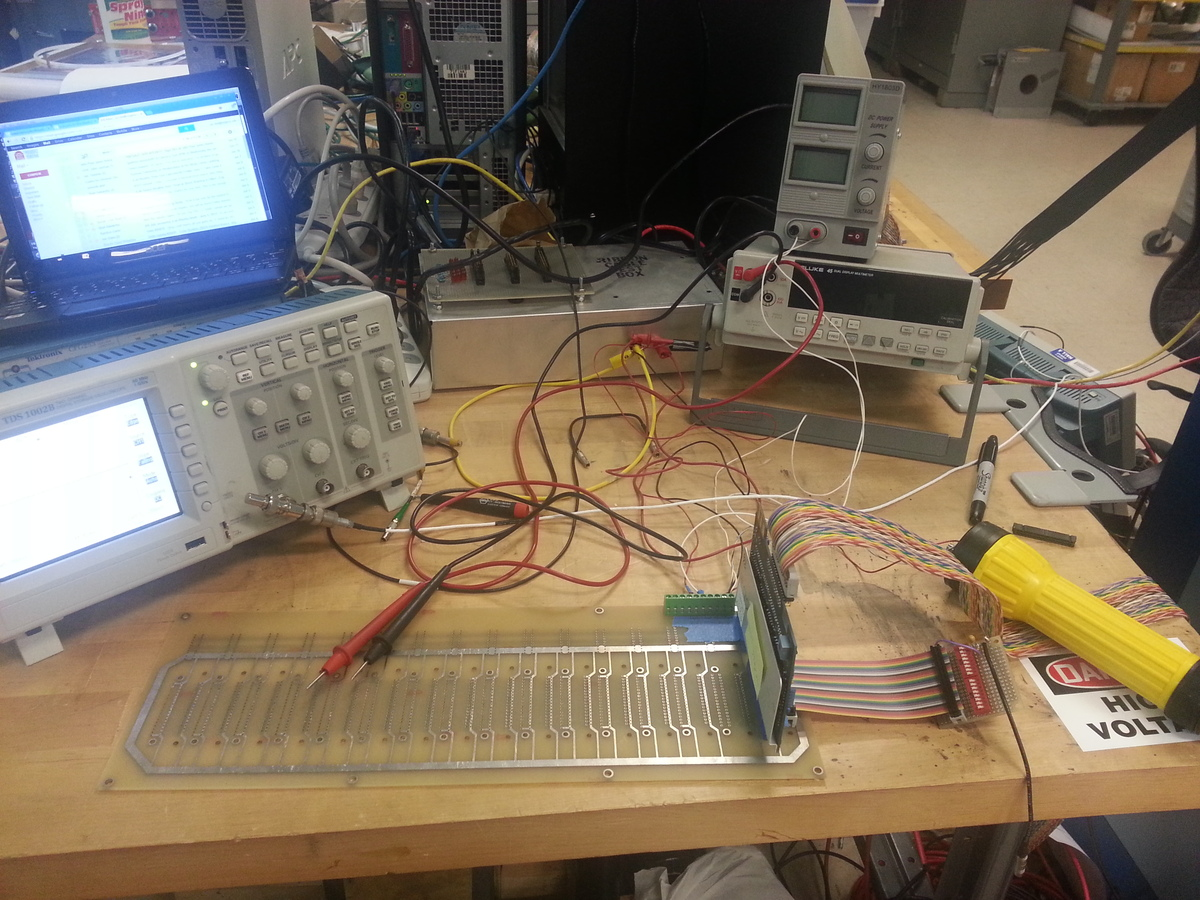
\includegraphics[height=3in]{Figure5.jpg}
  \caption{The (mostly) complete setup. Should give a good idea of what it will look like when assembled. To avoid confusion, if you're using our equipment it's worth noting the small switchboard is flipped upside-down in the final assembly because of some grounding problems}
  \label{fig:assembly}
\end{figure}
\begin{figure}[6]
  \centering
  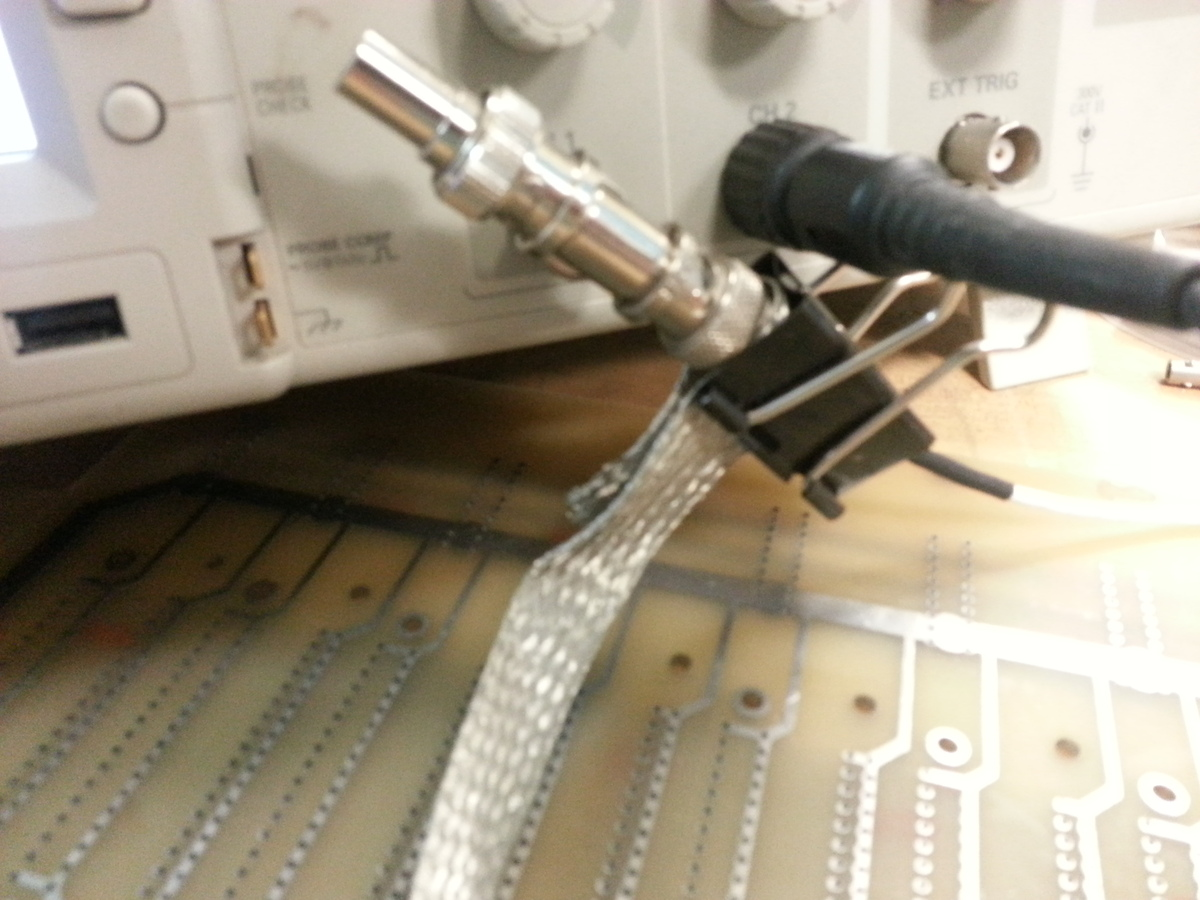
\includegraphics[height=3in]{Figure6.jpg}
  \caption{We had to ground the cable to the oscilloscope as well as the input through the attenuators on the switchboard with webbing to cut out noise. The second input on the scope is a voltage probe we used to check continuity.}
  \label{fig:grounding}
\end{figure}
\begin{figure}[7]
  \centering
  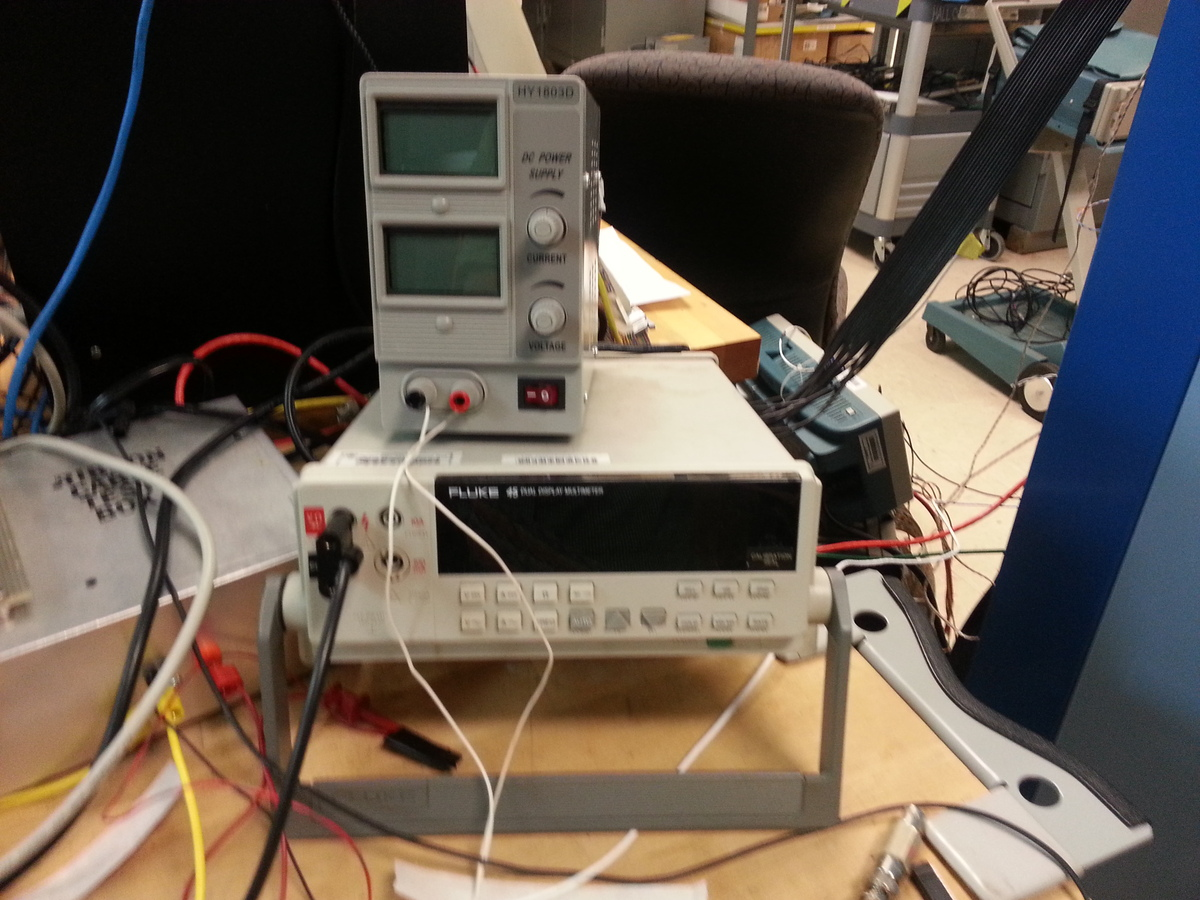
\includegraphics[height=3in]{Figure7.jpg}
  \caption{The large box on the bottom is the dedicated voltmeter we wired to the threshold voltage to monitor its level. The smaller device resting on it is the positive voltage source, putting out +5 volts}
  \label{fig:voltmeter}
\end{figure}
\begin{figure}[8]
  \centering
  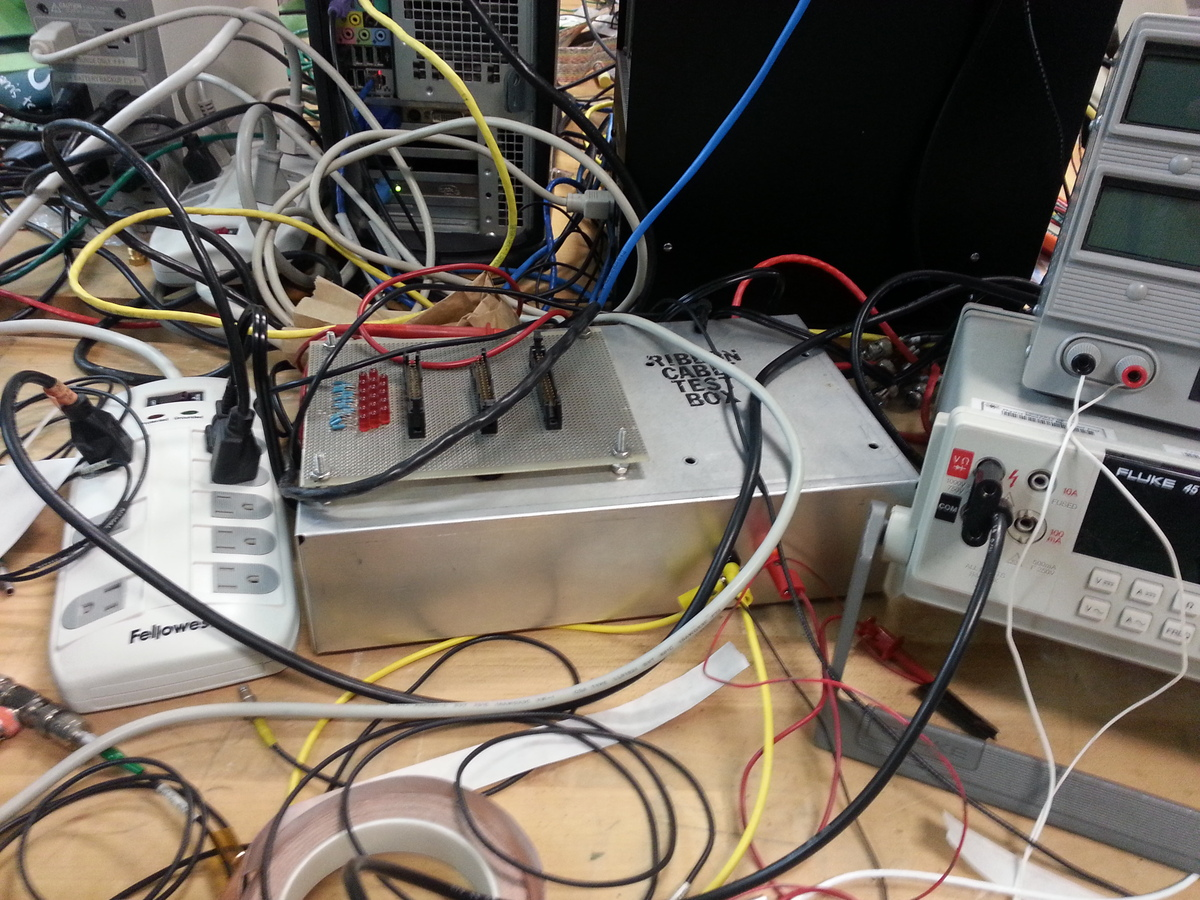
\includegraphics[height=3in]{Figure8.jpg}
  \caption{This large contraption is the negative voltage source, giving off -5 volts}
  \label{fig:negative}
\end{figure}
\begin{figure}[9]
  \centering
  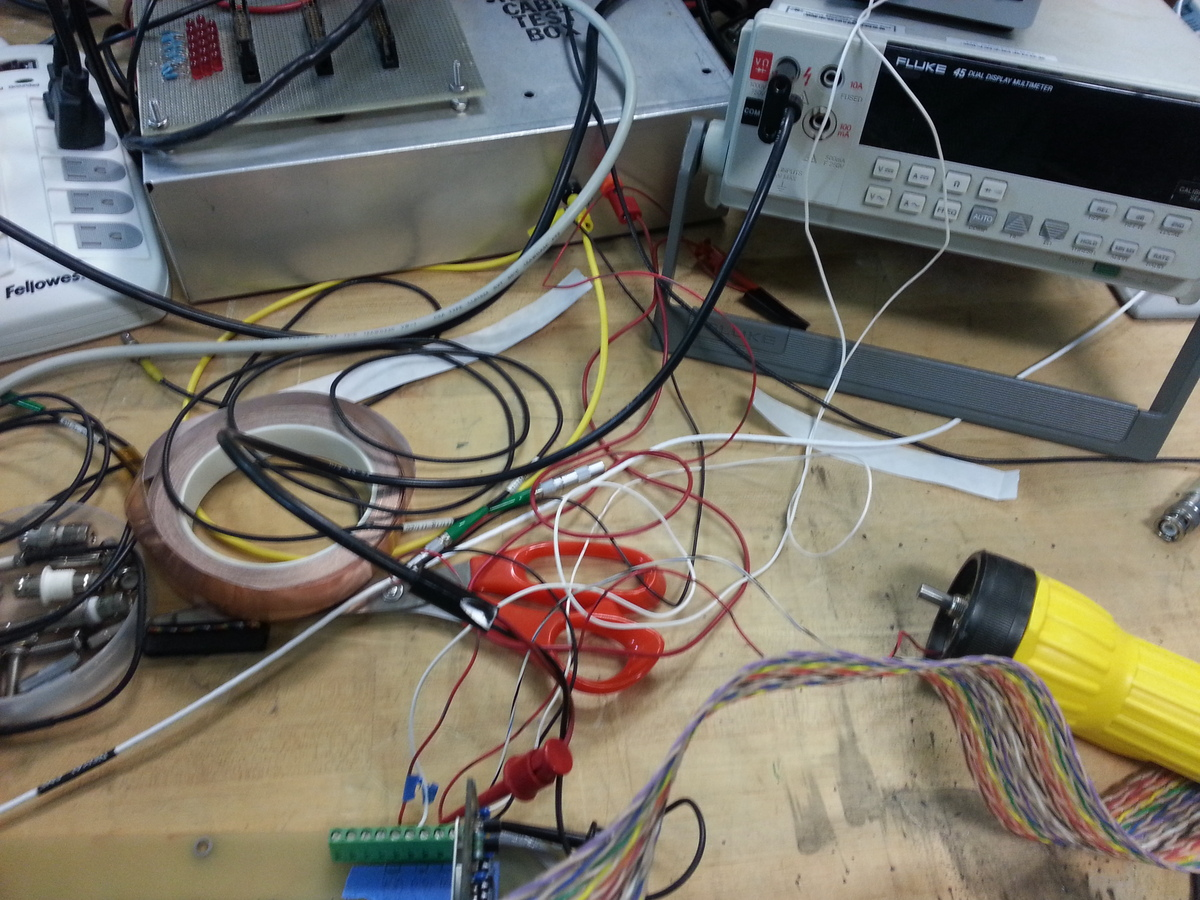
\includegraphics[height=3in]{Figure9.jpg}
  \caption{All the voltage sources together. The flashlight on the right is modified to be our threshold source, generating between 0 and +3 volts}
  \label{fig:whatamess}
\end{figure}
\begin{figure}[10]
  \centering
  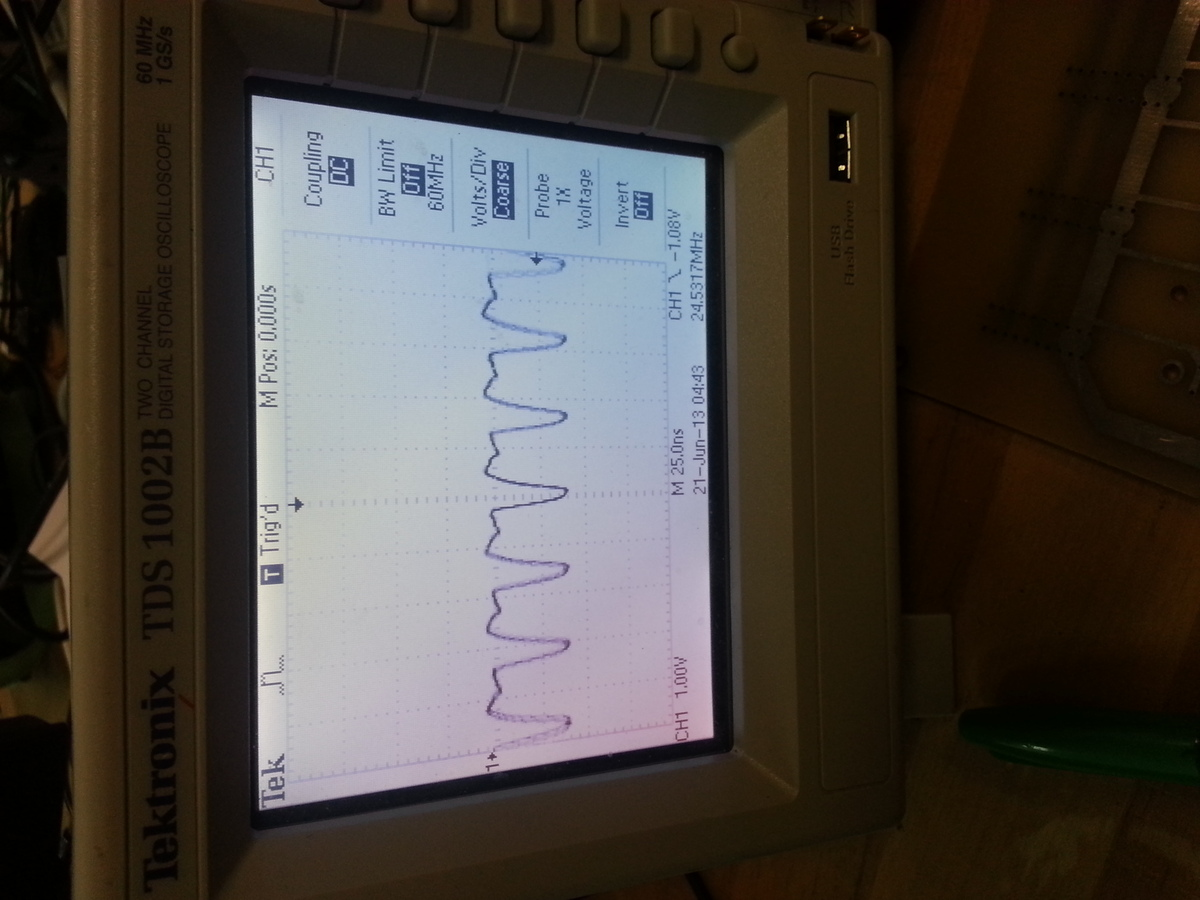
\includegraphics[height=3in, angle = -90]{Figure10.jpg}
  \caption{This is beyond the noise floor: when all the card triggers on is noise that would normally be discriminated out by the threshold voltage. Before you get to this point, you should be seeing flickers of stray pulses while the actual pulse is still somewhat defined.}
  \label{fig:noise}
\end{figure}
\begin{figure}[11]
  \centering
  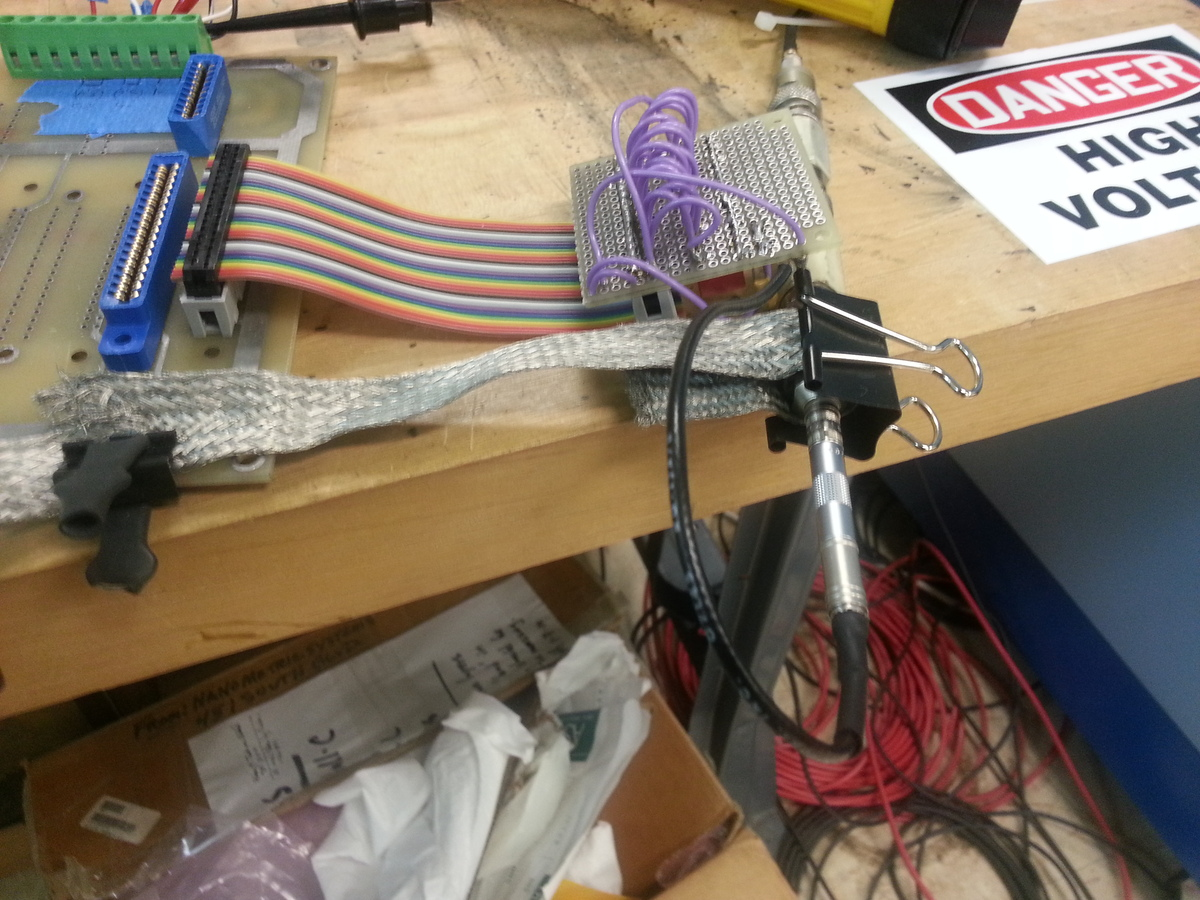
\includegraphics[height=3in]{Figure11.jpg}
  \caption{This where the input runs into the board. You can see the cable from the pulse generator running through the two attenuators. At the end of the second attenuator, you can see where the board cable plugs in in and where we had to ground the connection to the common ground on the large circuit board}
  \label{fig:input}
\end{figure}
\begin{figure}[12]
  \centering
  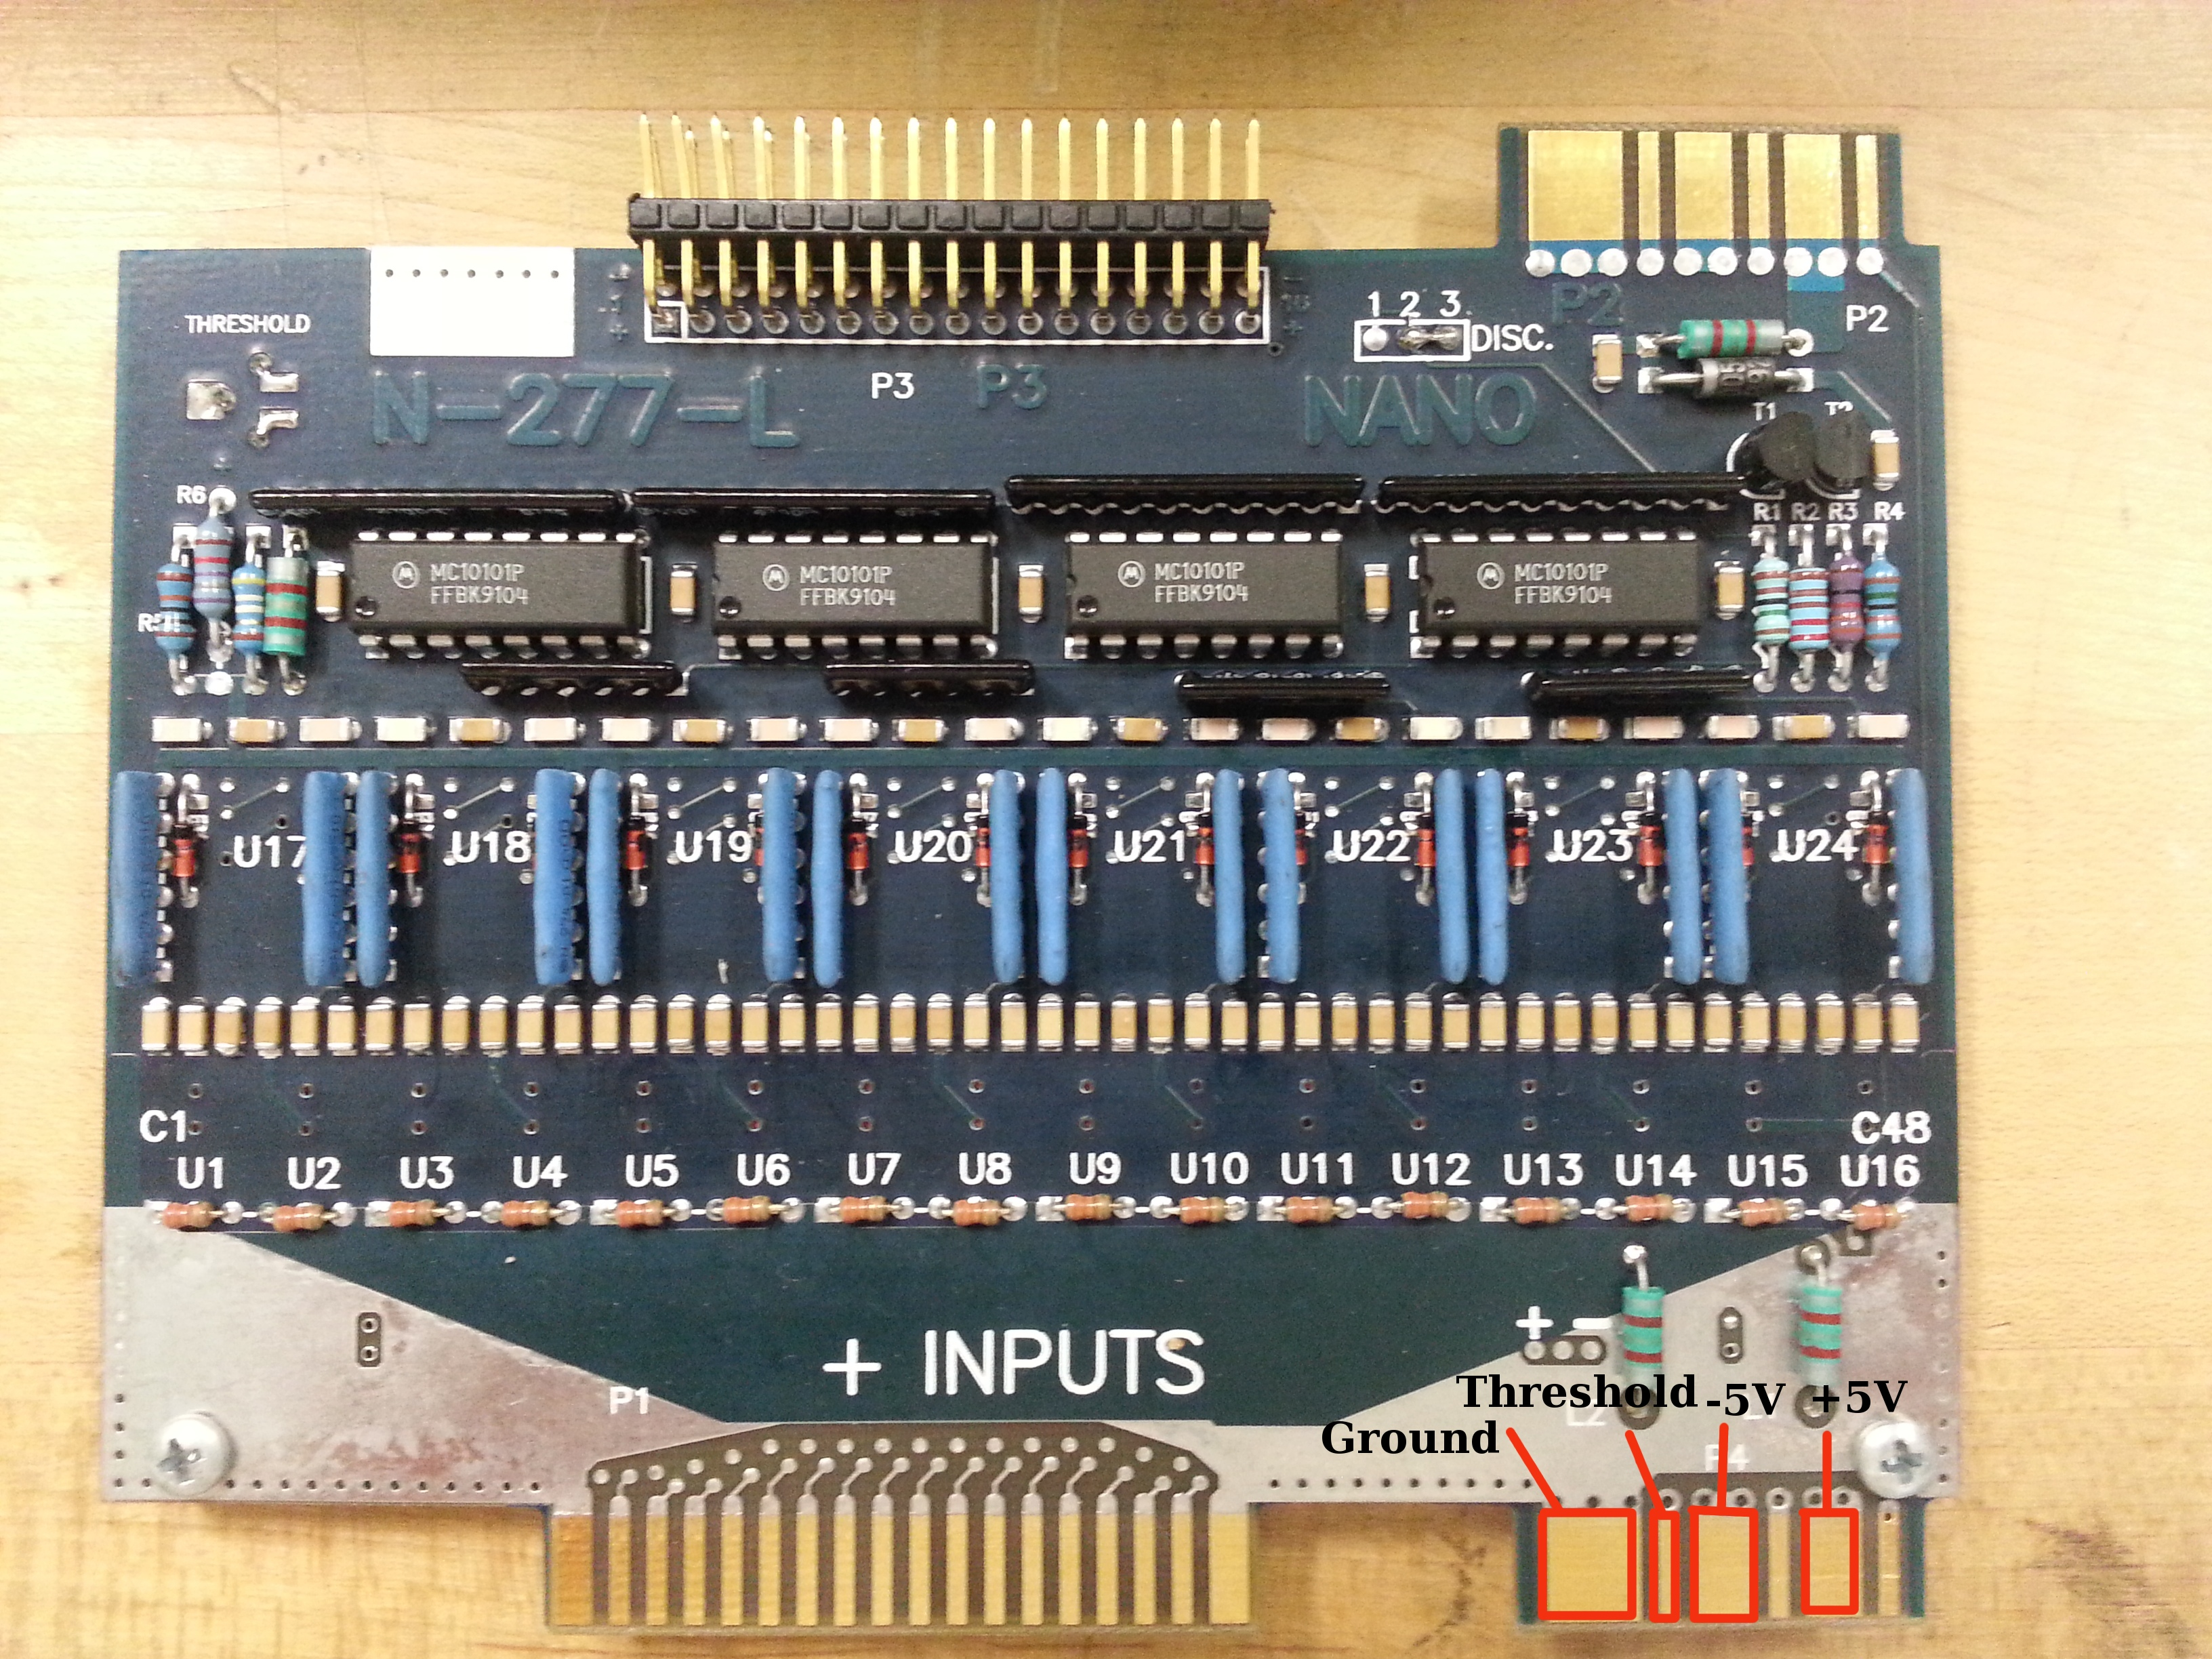
\includegraphics[height=3in]{Figure12.jpg}
  \caption{This is one of the cards we tested. Note that the pins have been highlighted and labeled with the respective voltage each should receive.}
  \label{fig:card}
\end{figure}

\begin{figure}[13]
  \centering
  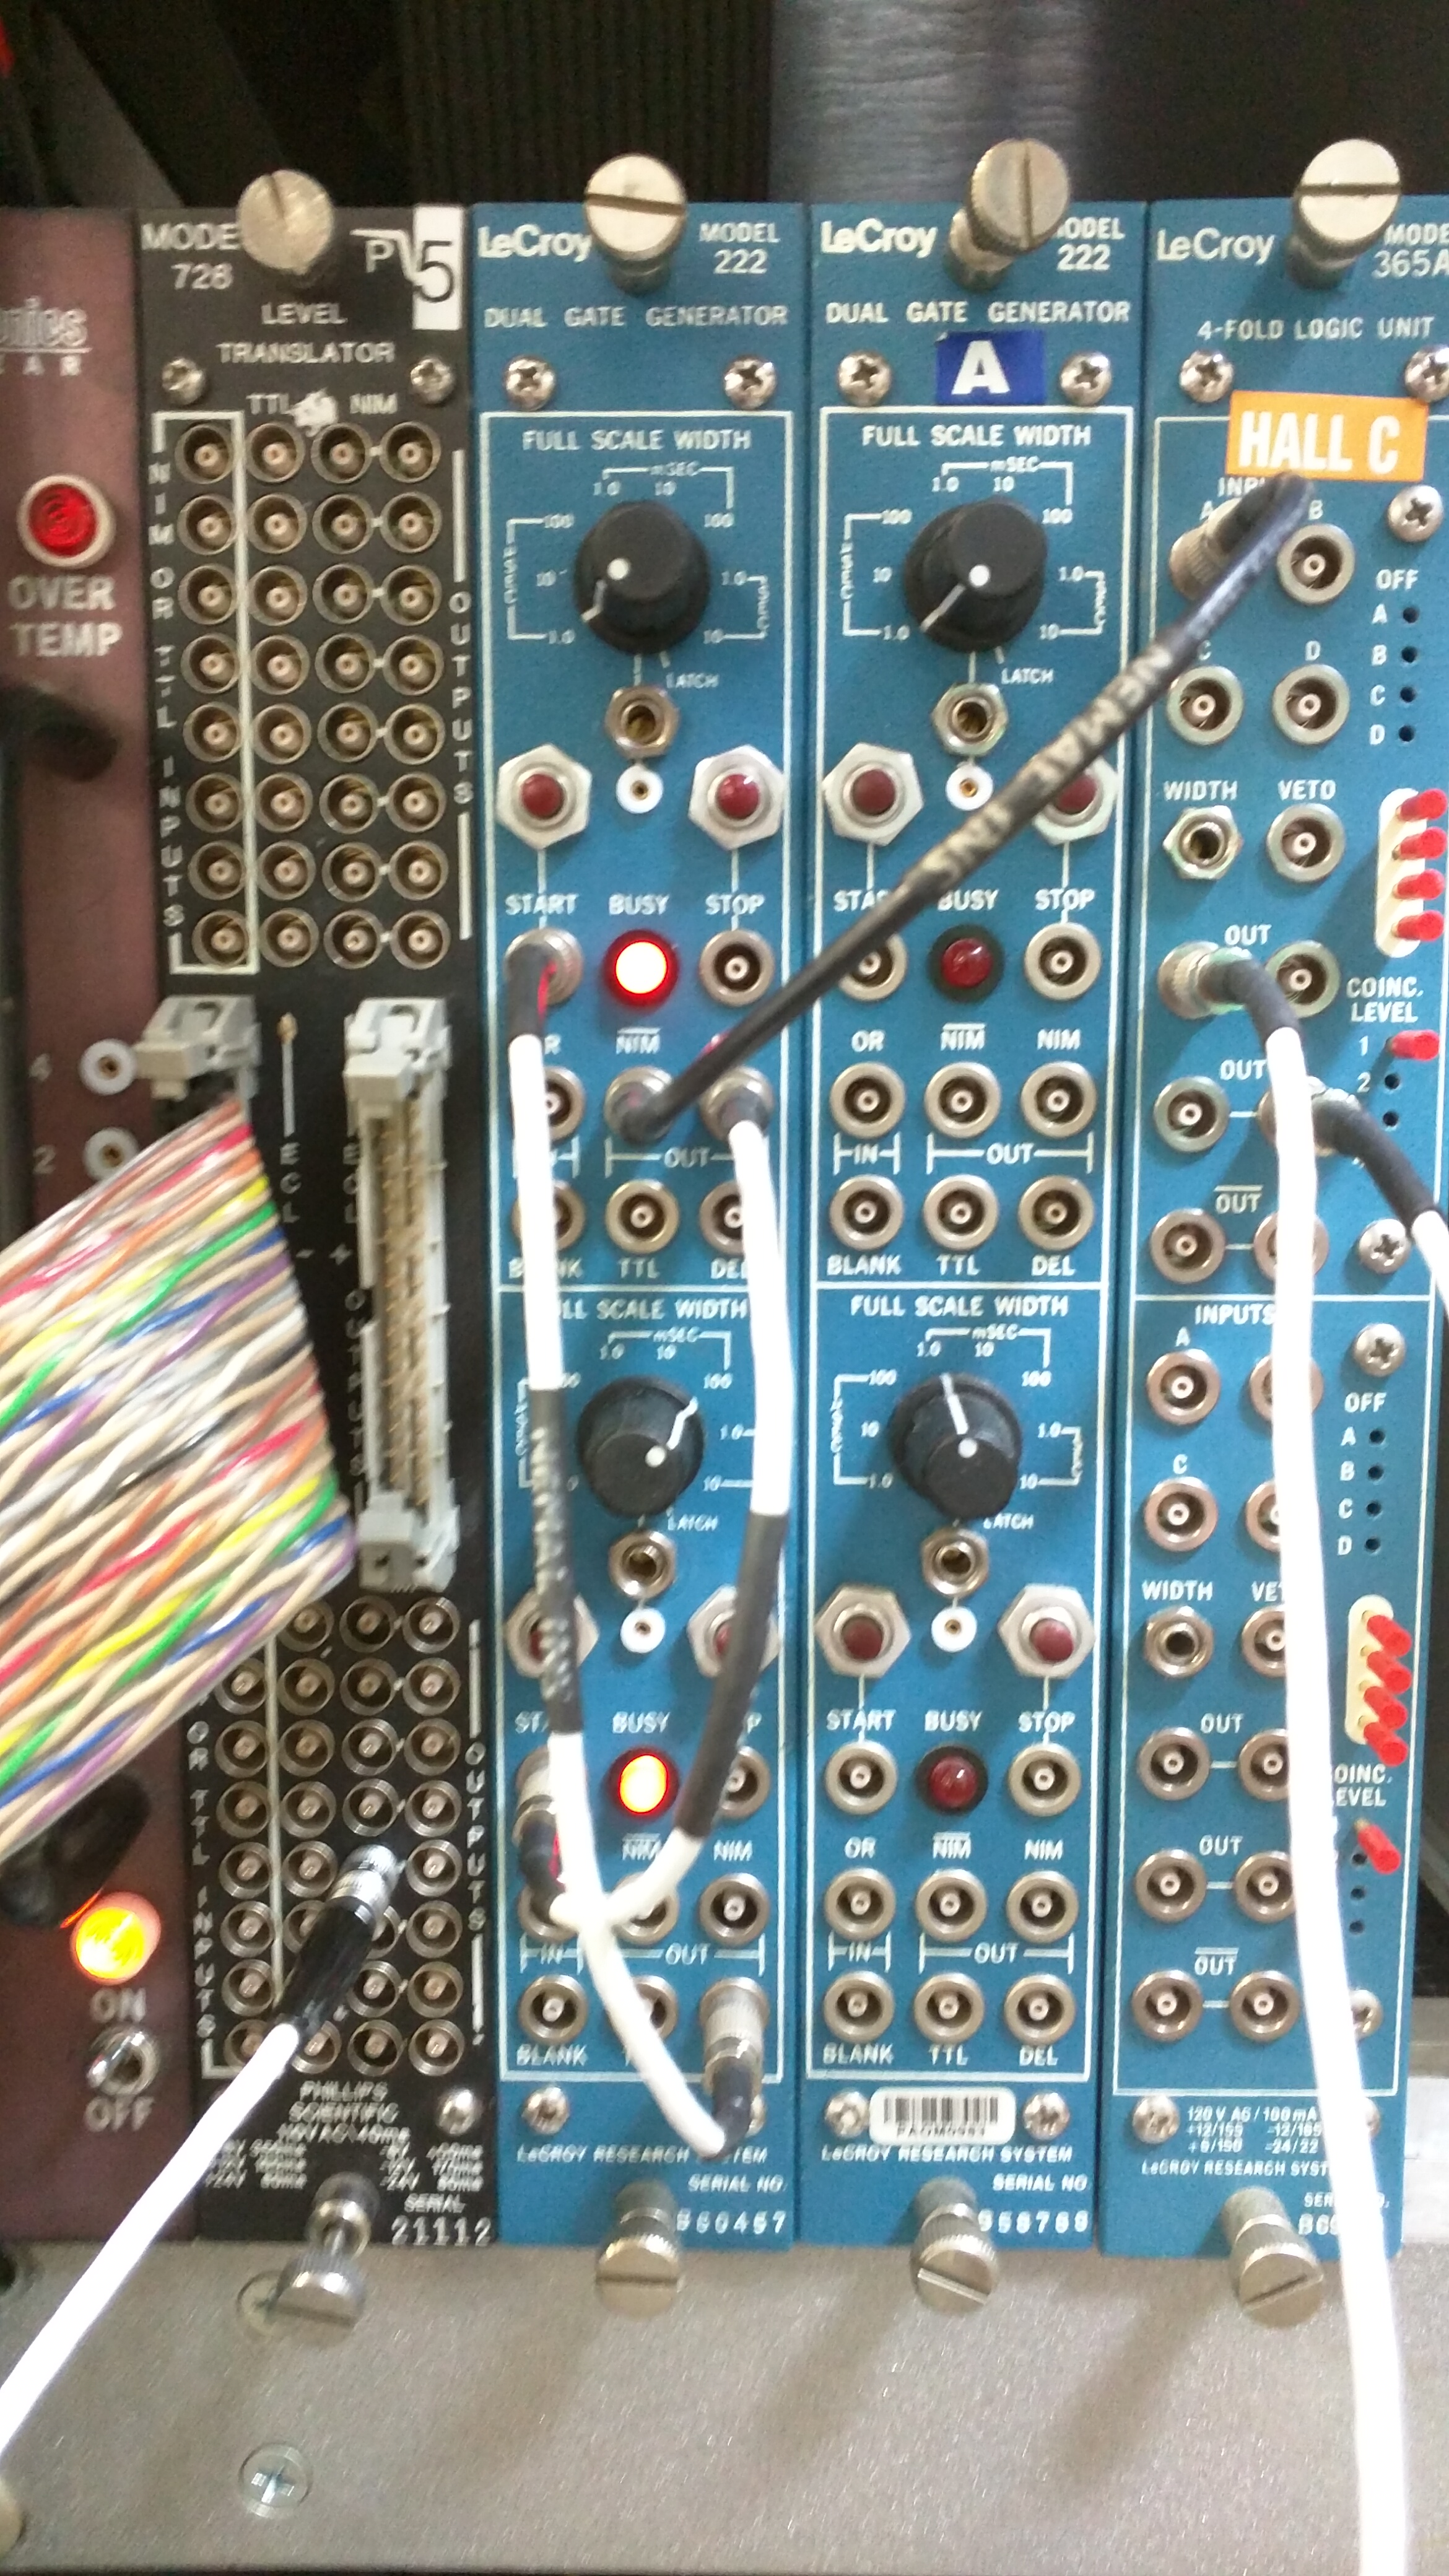
\includegraphics[height=3in]{IMG_20150715_153904.jpg}
  \caption{This is the dual gate generator creating input pulses of 45mV at 100Hz.}
  \label{fig:generator}
\end{figure}

\begin{figure}[14]
  \centering
  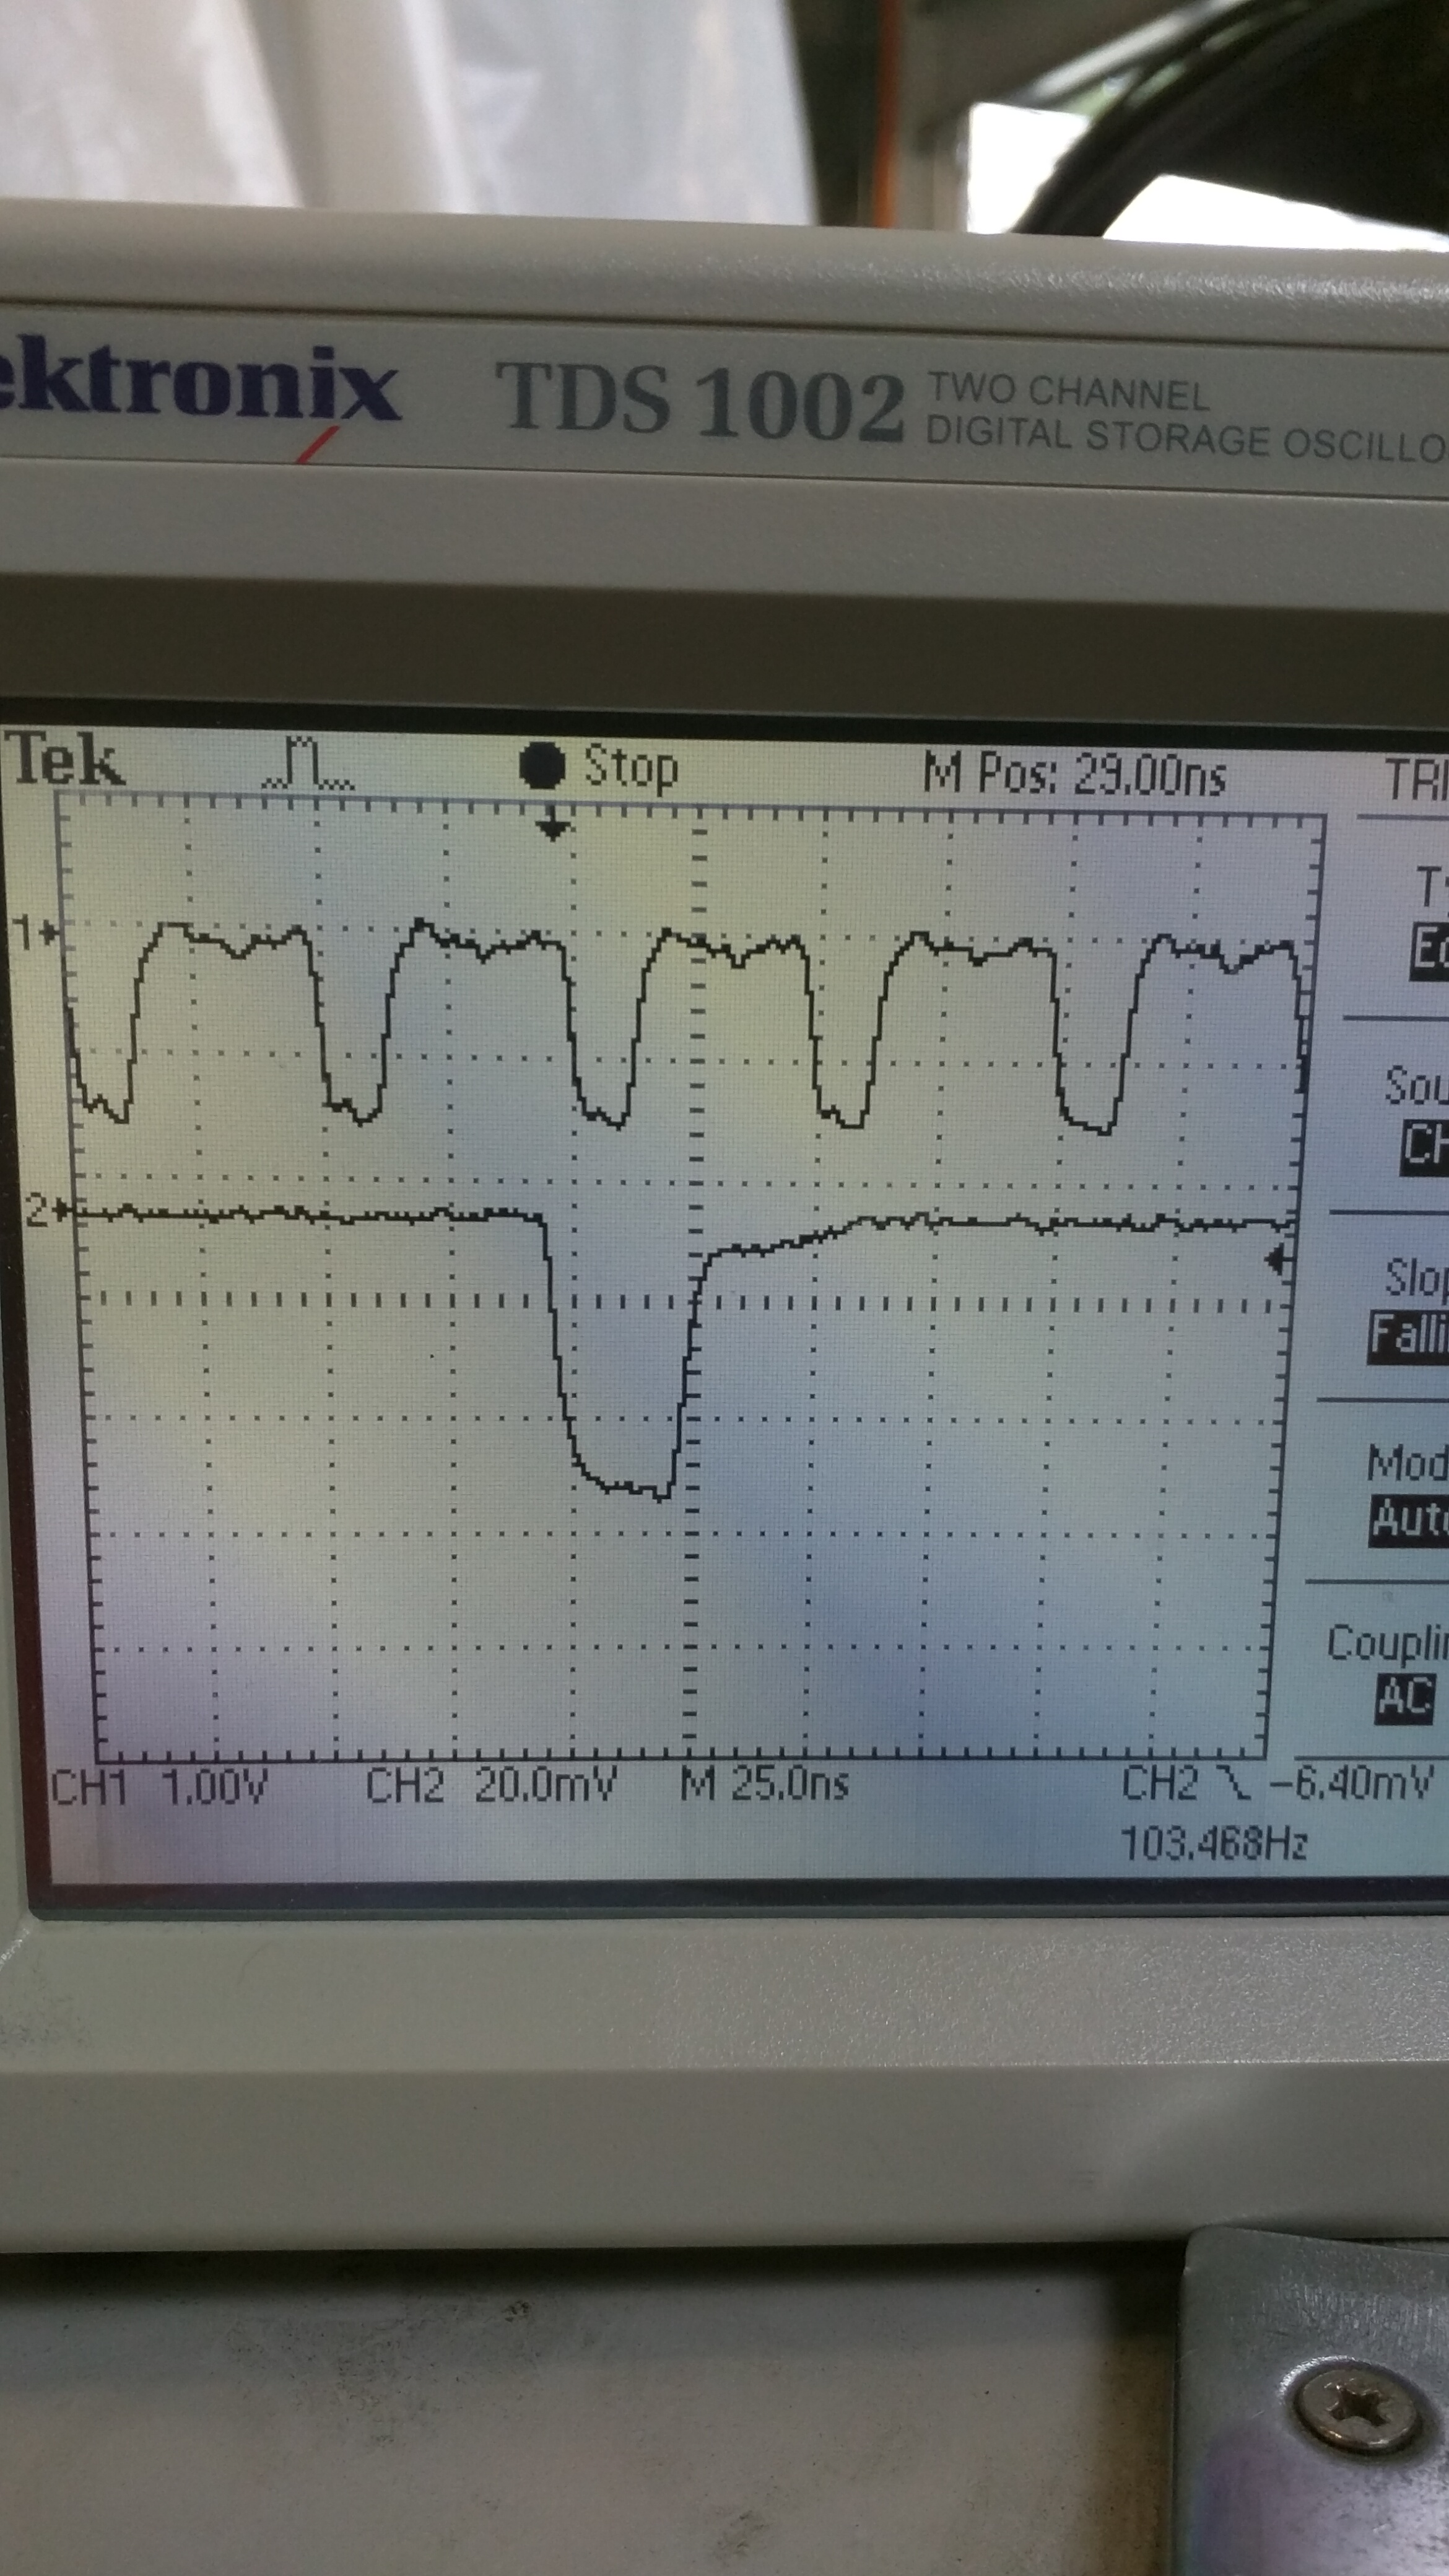
\includegraphics[height=3in]{IMG_20150715_154938.jpg}
  \caption{This shows the noise signals from the discriminator card in channel 1, and the 100Hz signals from the generator in channel 2}
  \label{fig:noise2}
\end{figure}\begin{figure}[15]
  \centering
  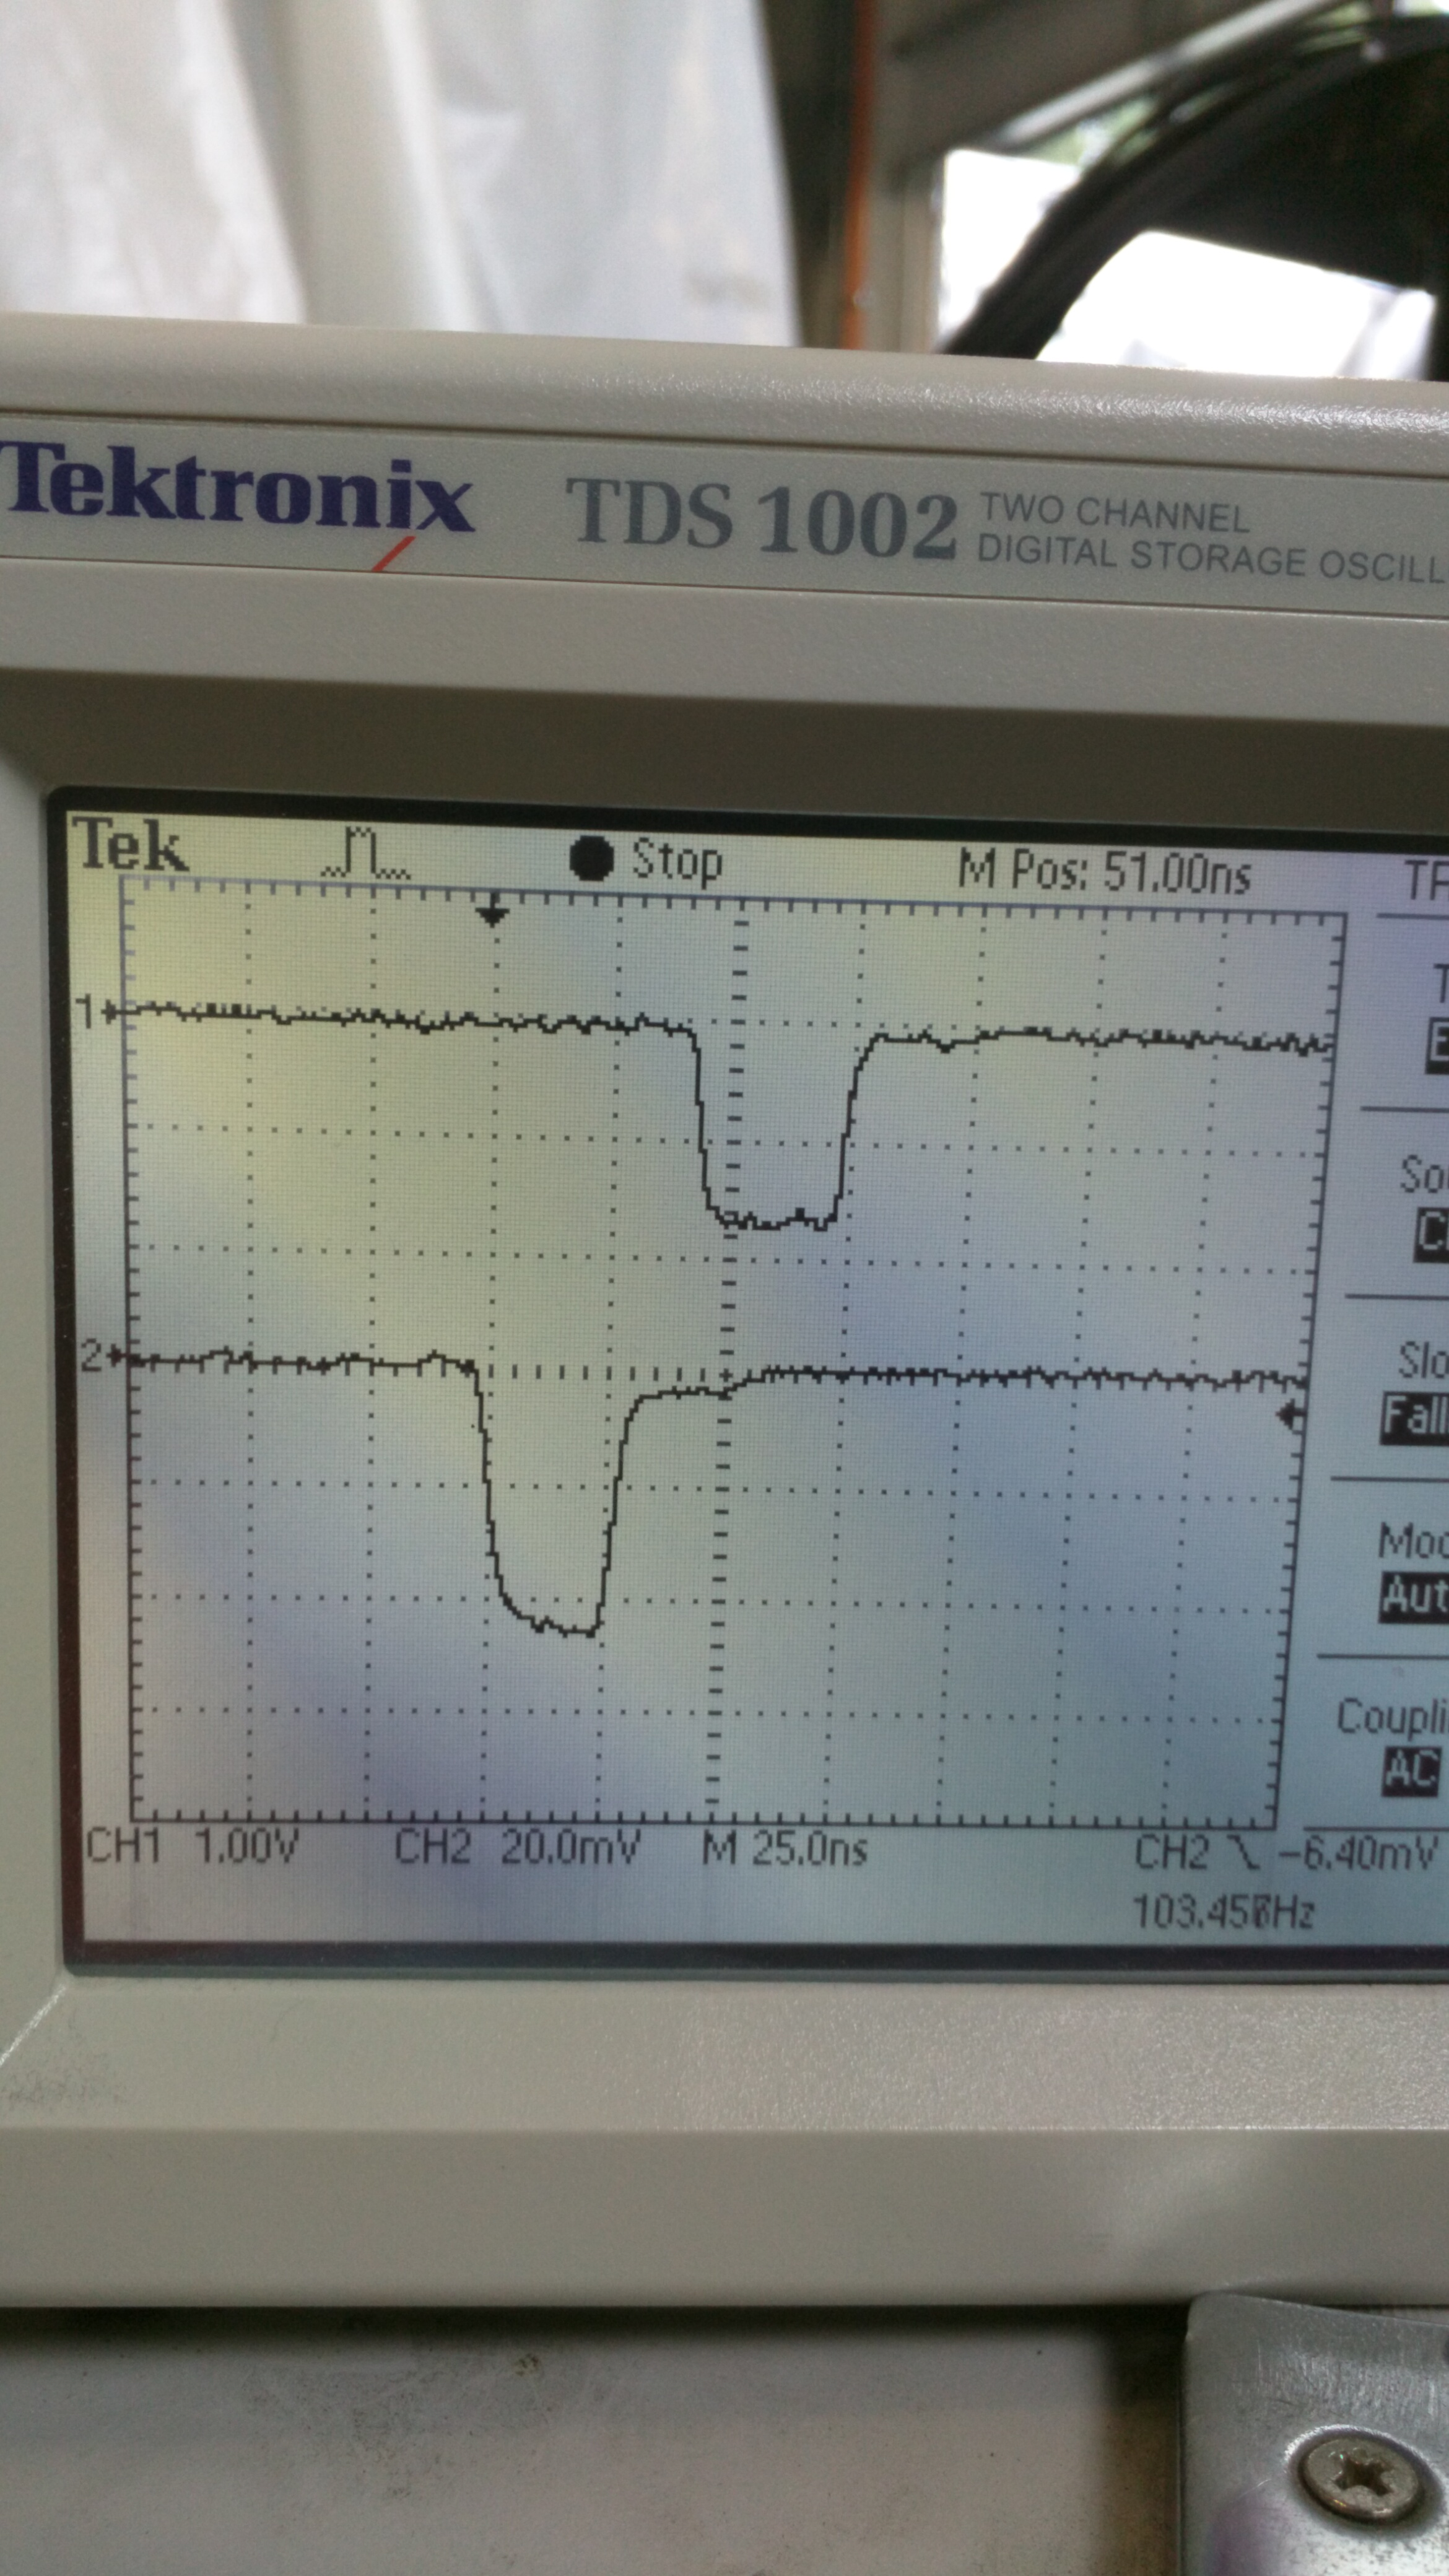
\includegraphics[height=3in]{IMG_20150715_155119.jpg}
  \caption{Channel 1 shows the discriminated pulses coming from the card at 100Hz, }
  \label{fig:discriminated}
\end{figure}

To test a discriminator card, first ensure you have the proper equipment. For our setup, we had three voltage sources, an oscilloscope, a pulse generator, a voltmeter, a scaler, and a NIM signal box. The three voltage sources will plug into the common ground on the circuit board and their respective pins corresponding to card outlined in Figure~\ref{fig:card}. For the cards we tested in particular, we needed +5 volts plugged into the 6th slot on the circuit board, linked to the 8th and 9th pins on the card. We plugged -5 volts into the 5th slot on the circuit board, linked to the 5th and 6th pins on the card, and the threshold voltage went into the 3rd slot on the board and connected to the 4th pin of the card. See Figure~\ref{fig:bus}. 

There exists a small circuit board that accepts the input pulse from the pulse generator. Connect this small circuit board with its ribbon cable to the larger board for the discriminator cards. The keys on the ribbon cable have been aligned according to the direction the ground and signal need to run respectively, and it should fit so that the small board is upside-down as pictured in Figure~\ref{fig:input}. Once everything is assembled, you are ready to test the cards.

Set the pulse generator to 210 millivolts, 100 hertz, and 25 nanoseconds wide. It will run through two attenuators linked together, a 6 decibel and a 14 decibel unit, as pictured. After the signal has been attenuated, a probe linked to the oscilloscope should reveal an input pulse of approximately 3 millivolts. Now connect the attenuated signal to the small circuit board and ensure that all the small switches are in the ``on'' position. Additionally, ensure that the connection between the signal and the small board and the connection from the NIM box to the oscilloscope (see Figure~\ref{fig:grounding}) are well grounded. We had some trouble with interesting noise until we connected them to the common ground on the bigger circuit board. Insert a discriminator card into the larger board and using a second ribbon cable connect the top bus on the card to the NIM signal board. In my tests, I then ran the signal from channel three of the NIM module to the first input on the oscilloscope. Set the oscilloscope to trigger on channel one (the channel the card signal feeds) at about -1 volt. First activate the threshold voltage, set to +2 volts. Our threshold voltage generator is the modified flashlight in Figure~\ref{fig:assembly}. Turn on the other two voltage sources. A logic pulse around -2 volts should appear from the card on the oscilloscope. 

From one channel on the NIM module (I chose channel four), run a cable into the left input of the scaler. Run another line from the pulse generator into a TTL module to convert the TTL signal to NIM. Then from that module, link the pulse into the right input of the scaler. Turn the small dial on the scaler to the ``3'' position, as pictured in Figure~\ref{fig:scaler}. This means that the scaler will compare the counts from the test source (the discriminator card) to $10^3$ (or 1000) counts from the input source (the pulse generator). Since the pulse generator runs at 100 hertz, this will be 10 seconds. Thus, to convert the result of the scaler back to hertz, simply divide by 100. Using the scaler, determine rate of the signal from the card as compared to the input pulse. Just hit the ``gate'' button and it will begin counting. The counts should be identical at the 2 volt threshold. 

Now using the oscilloscope, check each channel on the card to make sure it is producing a good signal. Often with this test, the pulse will cause some channels to fire twice, making the signal appear wider than on other channels, so be aware. When I ran through the tests, channel 9 liked to show no signal until I raised the pulse generator to 230 or 250 millivolts. This was a common pattern with most cards, so I attribute it to the equipment (i.e., don't worry about it). Because of this quirk, whenever you see a dead channel make sure it's actually dead by raising the amplitude of the pulse generator by several hundred millivolts. Now, turn the threshold voltage to 3 volts and run the scaler again. Once more, the counts from the card and the pulse generator should be identical.

After recording this rate, we want to find the noise floor-- the point where the card starts firing on background noise instead of on input pulses. This means that the voltage threshold must be lowered. I'll pause and explain what I mean by threshold voltage: this is an voltage input to the card that tells the card when to display a logic pulse. The card contains an amplifier to raise the tiny voltages it will receive in the wire chamber to readable levels. When the signal it amplifies is above the threshold voltage, it will display a logic pulse. Thus, we want the threshold to be low enough to be triggered by the input pulse and high enough to filter out background noise. We want to find the ``noise floor'' to see exactly where we read noise instead of legitimate signals. So, watching the oscilloscope, lower the threshold voltage until you see random pulses that do not align with the card's normal logic pulse. The oscilloscope should appear as in Figure~\ref{fig:noise}. Record the noise floor and tune the threshold back to +2 volts. 

We now need to evaluate cross talk between channels on the card. Cross talk happens when the signal going into one channel on the card ``overflows'' into the channels adjacent to it. In my tests, I plugged channel four from the card signal into the scaler while channel three ran to the oscilloscope. You want to disable the channel going into the scaler, so turn the switch on the small circuit board to the off position for that particular channel (in my case, this was channel four). See Figure~\ref{fig:switches}. Now run the scaler again. The count should be under 20 hertz, otherwise the cross talk rate is too high for the card to function reliably. Turn the threshold to 3 volts and repeat the test. Record your results.

At this point, you've run all the tests to check the functionality of a discriminator card, well done. Now repeat 80+ times, and you're good to go!



For our setup, at threshold of -2 Volts only a few channels per discriminator card  produced logic pulses. Many of the channels did not begin to produce pulses until a threshold range of about 400-800mV. This led to issues with several cards due to the noise floor being at a similar voltage(~200-500mV), or even higher than that of the threshold. For example, channel 16 tended to have a lower threshold than the other channels across all cards. The 16th channel was used as the basis for initially deterining each card's threshold and noise floor. So, we measured the threshold voltage of channel 16 by observing when its pulses stopped appearing on the oscilloscope. This was determined to be the maximum threshold. Then we checked the rest of the channels to make sure that they got a pulse at that voltage. If they did, then the card was determined to be good. Otherwise, if one or more of the channels did not receive a pulse, then we would attempt to find the pulse at a lower threshold. If we did, then that was made the new maximum threshold. If we could not find the pulse, then the card was thrown in the bad column. 


To produce pulses at 100Hz and 25ns widths, we had to use two delays from a dual gate generator ass seen in the figure. The gate generators could then directly adjust the width and spacing of the pulses smaller than the pulse generator. The pulse amplitude from the rig was then attenuated to 45mV, rather than the 210mV previously indicated. With this generator and the 6db and 14db attenuators, the input signals were at the desired amplitude of ~3mV.



\end{document}
